\documentclass{article}
\usepackage[utf8]{inputenc}
\usepackage[a4paper, total={6.4in, 8.53in}]{geometry}
\usepackage{amsmath, tikz, amsfonts, bbm, mathrsfs, graphicx, amssymb, amsthm, hyperref, centernot, enumerate, bbm, xcolor, lmodern, mathdots, amsfonts, graphicx}
\usepackage{subcaption}
\usepackage{multirow}
\usepackage{algorithm}% http://ctan.org/pkg/algorithm
\usepackage{algpseudocode}% http://ctan.org/pkg/algorithmicx
\usepackage{float}
\usepackage{hyperref}


\title{MAT1856/APM466 Assignment 1}
\author{Lisa Yu, Student \#: 1005786366}
\date{February 6th, 2020}

\begin{document}

\maketitle

\section*{Fundamental Questions - 25 points}

\begin{enumerate}
    \item \hfill
    \begin{enumerate}
        \item Governments issue bonds instead of just printing more money because in some countries the government is not allowed to print money (only the central bank can) and also to avoid inflation caused by increased money supply and limited goods since issuing bonds does not increase the supply of money.
        \item Regardless of market conditions, the yield curve tends to have a flatter tail because investors are more uncertain about the more distant future, but if the curve flattens (or even inverts), this could be because short term interest rates increase more than the long term interest rates due to increased volatility in the short term market or that investors expect long-term interest rates to drop due to slowed economic growth and could signal a recession \cite{flatyield2023}. 
        \item Quantitative Easing (QE) is a monetary policy where the central bank buys government bonds and other securities on the open market to increase the supply of money (more liquidity), lower interest rates, and increase economic activity; during the COVID-19 pandemic, the Fed used QE to increase its holdings to account for 56 percent of the Treasury issuance of securities through the first quarter of 2021 and eventually claimed that it would buy as much securities as needed to support smooth market functioning \cite{milstein2022fed, team2023quantitative}.
    \end{enumerate}
    \item The list of bonds I have chosen to construct the yield, spot, and forward curves are CAN 0.25 AUG 23, CAN 2.25 MAR 24, CAN 1.5 SEP 24, CAN 1.25 MAR 25, CAN 0.5 SEP 25, CAN 0.25 MAR 26, CAN 1.0 SEP 26, CAN 1.25 MAR 27, CAN 2.75 SEP 27, CAN 3.5 MAR 28. I chose these because their maturity dates are closest to 6 months apart so their cash flows match most closely. This way, I can approximately use the previous zeros (spots) calculated using bootstrapping of the bonds with earlier maturity dates to discount the cash flows of the bonds with later maturity dates. Notice that I skipped the CAN 1.75 MAR 23 bond since that is approximated to have a time to maturity of 0 years. I also picked the bonds with the most similar coupon rates (0.25-3.5 percent) and issuance dates (2018-2022) because it makes the bonds more comparable (more of the same "class" or "market" of bonds). Specifically, bonds with a much higher coupon payment has a larger reinvestment risk since the yield to maturity assumes that the investor reinvests the coupon payments back at a ytm rate. Very different issuance dates of the bonds may effect the liquidity of the bond and introduce a liquidity risk premium in the bond prices because investors are more willing to buy an on-the-run bond.
    \item PCA decomposes the covariance matrix to a new set of independent vectors (eigenvectors) that capture the most variability in the data. Larger eigenvalues mean more variability along that direction (the eigenvector explains more variance in the data). In the case of the stochastic processes, the eigenvalues indicate how much the stochastic curve changes in the direction of each eigenvector. The eigenvectors in the case of the stochastic processes describe the directions that the stochastic curve changes the most (such as constant shifts in all the processes, or slopes and curves).
\end{enumerate}



\section*{Empirical Questions - 75 points} 

\begin{enumerate}
\setcounter{enumi}{3} 
    \item \hfill
    \begin{enumerate}
        \item  
            Using the bond data collected, we can construct the yield to maturity curve \cite{hayes2023yield} (Figure 1) by solving for the IRR of the present value equation of the bonds using Python (see code in repository). The graph uses linear interpolation to interpolate the missing values since that is the easiest method, provides smooth estimates for values between observed points, and is robust to outliers. (We use the same interpolation method for the spot and forwards curve construction.) Notice that the yield curve is inverted and peaks at 1 year. This is because people expect the long term interest rate to be lower than the short term rate perhaps because short term interest rate may be increased further to combat the current inflation and then later decreased as inflation and economic growth slows (this explains the peak at 1-yr). This signifies a recession. 
            
            \begin{figure}[h!]
            \centering
            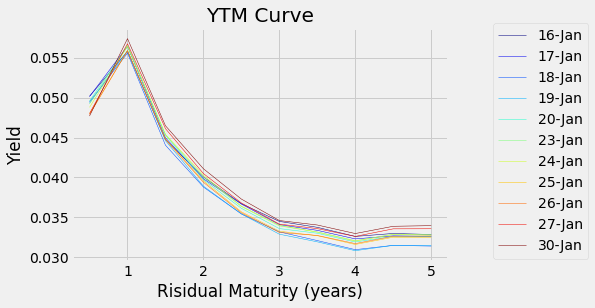
\includegraphics[width=0.5\textwidth]{YTM_curve.png}
            \caption{YTM Curve}
            \label{fig:YTM Curve}
            \end{figure}
        \item Using the bond data collected, we can construct the spots curve \cite{hayes2022spot} (Figure 2) through bootstrapping (Algorithm 1). Notice that the spot curve values are slightly lower than that of the ytm but follows the same general shape as the yield curve for the same reasons as explained in part (a). The spots being lower than the ytm is usually the case for inverted yield curves because in general, assuming annual coupon payments, the $ytm_n$ is the rate such that $$Price = \frac{c}{1+ytm_n} + \frac{c}{(1 + ytm_n)^2} + ... + \frac{c + 100}{(1+ytm_n)^n}$$ and $spot_n$ is the rate $z_n$ such that $$Price = \frac{c}{1+z_1} + \frac{c}{(1 + z_2)^2} + ... + \frac{c + 100}{(1+z_n)^n}$$ so $ytm_n$ can be thought of as some sort of "average" of the $z_1$, $z_2$, ... $z_n$'s and since $z_1 > z_2 > ... > z_n$ (because the yield curve is inverted), $ytm_n$ must be larger than $z_n$. 
            \begin{figure}[h!]
            \centering
            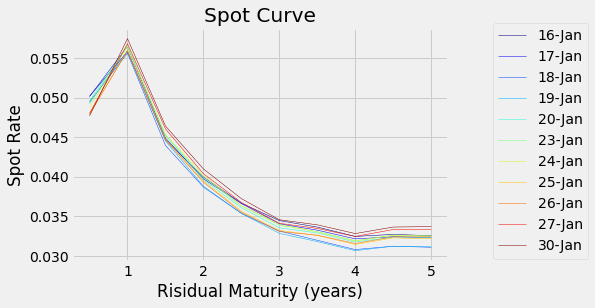
\includegraphics[width=0.5\textwidth]{spots_curve.png}
            \caption{Spots Curve}
            \label{fig:Spots Curve}
            \end{figure} 

            \begin{algorithm}[H]
              \caption{Deriving Spot Curve}\label{spot}
              \begin{algorithmic}[1]
                \Function{GetSpotCurve}{$prices, coupons$}\Comment{get the spot rates for one day of bond data}
                  \State $zeros\gets []$ \Comment{initialize empty zeros list}
                  \State $z_1\gets (\frac{\frac{coupons[1]}{2} + 100}{prices[1] - \frac{coupons[1]}{2}} - 1) * 2$ \Comment{calculate the first zero}
                  \State append $z_1$ to $zeros$
                  \For{\texttt{$i$ in $[2, 3, ..., 10]$}} \Comment{for each of the maturity dates}
                    \State $price \gets prices[i]$
                    \State $coupon \gets coupons[i] / 2$
                    \State $frontPV \gets \Call{GetPV}{coupon, i-1, zeros}$ \Comment{get PV for all CF except for last}
                    \State $z \gets (\sqrt[i]{\frac{coupon + 100}{price - frontPV}} - 1) * 2$
                    \State append $z$ to $zeros$
                  \EndFor
                  \State \textbf{return} $zeros$
                \EndFunction
                \[\]
                \Function{GetPV}{$coupon, nperiods, zeros$}\Comment{get the present value of all cash flows up to nperiods}
                    \State $pv \gets 0$
                    \State $pv \gets pv + coupon$
                    \For{\texttt{$i$ in $[1, 2, ..., nperiods]$}} \Comment{for each cashflow period}
                        \State $pv \gets pv + \frac{coupon}{(1 + \frac{zeros[i]}{2})^i}$
                    \EndFor
                    \State \textbf{return} $pv$
                \EndFunction
              \end{algorithmic}
            \end{algorithm}

        \item Using the bond data collected, we can construct the forward curve \cite{chen2022forward} by using our zero (spot) rates calculated earlier (Algorithm 2). Notice the relationship where the $(1 + \frac{zero_n}{2})$ equals the geometric mean of $(1 + \frac{forward_{0.5}}{2}), (1 + \frac{forward_1}{2}), ..., (1 + \frac{forward_n}{2})$. Also note that for any given day, the priced-in forward rates in 1 year (Figure 3b) is precisely the priced-in forward rates now (Figure 3a) shifted to the left by 1 year. In other words, the priced-in forward rate in one year for $n$ years ahead is the same as the priced-in forward today for $n+1$ years ahead because the market data has not changed. Notice that the forward rates follow a similar trend as the ytm and spots (for the same reason as explained above) but fluctuates more since they are the purest form of rates with no compounding and so they are more sensitive to the bond price, and because the 10 bonds that we picked are not perfect (they do not have the same coupon rate, issue date, etc.), the resulting forward rates fluctuates a bit more.
        
            \begin{figure}[H]
            \begin{subfigure}{0.5\textwidth}
            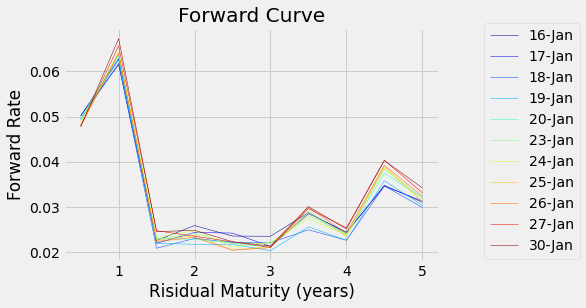
\includegraphics[width=\linewidth]{forward_curve.png}
            \caption{Forward Curve}
            \end{subfigure}
            \begin{subfigure}{0.5\textwidth}
            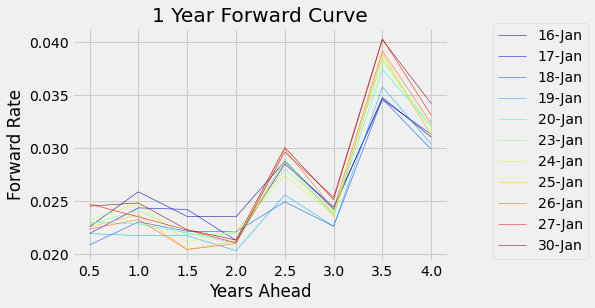
\includegraphics[width=\linewidth]{forward_curve_1.png}
            \caption{1 Year Forward Curve}
            \end{subfigure}
            \caption{Forward Curves}
            \label{fig:Forward Curves}
            \end{figure}

            \begin{algorithm}[H]
              \caption{Deriving Forward Curve}\label{forward}
              \begin{algorithmic}[1]
                \Function{GetForwardCurve}{$zeros$}\Comment{get the forward rates for one day of bond data}
                    \State $forwards\gets []$ \Comment{initialize empty forwards list}
                    \State $f_1 \gets zeros[1]$ \Comment{first forward is same as first zero}
                    \State append $f_1$ to $forwards$
                    \For{\texttt{$i$ in $[2, 3, ..., 10]$}} \Comment{for each of the maturity dates}
                        \State $factor \gets \Call{GetPreviousForwardsProduct}{forwards, i-1}$ 
                        \State $f = [((1 + \frac{zeros[i]}{2})^i * factor) - 1] * 2$
                        \State append $f$ to $forwards$
                    \EndFor
                    \State \textbf{return} $forwards$
                \EndFunction
                \[\]
                \Function{GetPreviousForwardsProduct}{$forwards, nperiods$} \Comment{get the product of all the (1 + forward rates)}
                    \State $factor \gets 1$
                    \For{\texttt{$i$ in $[1, 2, ..., nperiods]$}} \Comment{for each of the maturity dates}
                        \State $factor \gets factor / (1 + \frac{forwards[i]}{2})$
                    \EndFor
                    \State \textbf{return} $factor$
                \EndFunction
                \[\]
                \Function{GetOneYearForward}{$forwards$} \Comment{input is current year forwards}
                    \State \textbf{return} last 8 elements of $forwards$
                \EndFunction
              \end{algorithmic}
            \end{algorithm}

    \end{enumerate}
    \item See below for the covariance matrices of the YTM log returns (Table 1) and the 1-YR Forward log returns (Table 2).
        \begin{table}[H]
        \begin{minipage}{0.5\linewidth}
        \centering
        \caption{Covariance Matrix of YTM Log Returns}
        \begin{tabular}{|c|c|c|c|c|}
        \hline
        1.1111 & 0.9362 & 0.8522 & 0.8762 & 0.8711 \\ \hline
        0.9362 & 1.1111 & 1.0845 & 1.0362 & 1.0184 \\ \hline
        0.8522 & 1.0845 & 1.1111 & 1.0231 & 0.9974 \\ \hline
        0.8762 & 1.0362 & 1.0231 & 1.1111 & 1.1067 \\ \hline
        0.8711 & 1.0184 & 0.9974 & 1.1067 & 1.1111 \\ \hline
        \end{tabular}
        \end{minipage}
        \hfill
        \begin{minipage}{0.5\linewidth}
        \centering
        \caption{Covariance Matrix of 1-YR Forward Log Returns}
        \begin{tabular}{|c|c|c|c|}
        \hline
        1.1111 & 0.7794 & 0.4588 & 0.4337 \\ \hline
        0.7794 & 1.1111 & -0.0864 & -0.0925 \\ \hline
        0.4588 & -0.0864 & 1.1111 & 0.9293 \\ \hline
        0.4337 & -0.0925 & 0.9293 & 1.1111 \\ \hline
        \end{tabular}
        \end{minipage}
        \end{table}
    \item The first eigenvalue of the ytm covariance matrix shows that the first principal component explains 90 percent of the total variance and its first eigenvector represents the situation that all rates in the yield curve move in the same direction by relatively the same amount (level shift) (Table 3), while the first eigenvalue of the 1-YR forwards covariance matrix shows that its first princial component explains 54 percent of total variance and its first eigenvector represents the situation that all rates in the yield curve move in the same direction by relatively the same amount except for the 1-YR 2-YR rate which moves by a little bit less (Table 4) \cite{pca2023yield}.

        \begin{table}[H]
            \centering
                \begin{tabular}{llllll}
                    \hline
                    \multirow{5}{*}{Eigenvectors} & \multicolumn{1}{l}{-0.41040864} & \multicolumn{1}{l}{-0.89228493} & \multicolumn{1}{l}{0.10231514} & \multicolumn{1}{l}{0.15769443} & \multicolumn{1}{l}{0.0075125} \\
        
                    & \multicolumn{1}{l}{-0.46074175} & \multicolumn{1}{l}{0.02541976} & \multicolumn{1}{l}{-0.42663837} & \multicolumn{1}{l}{-0.77572515} & \multicolumn{1}{l}{-0.05745497} \\
        
                    & \multicolumn{1}{l}{-0.45077206} & \multicolumn{1}{l}{0.24491404} & \multicolumn{1}{l}{-0.60163085} & \multicolumn{1}{l}{0.5963938} & \multicolumn{1}{l}{0.13847894} \\
        
                    & \multicolumn{1}{l}{-0.45828112} & \multicolumn{1}{l}{0.27087663} & \multicolumn{1}{l}{0.39908526} & \multicolumn{1}{l}{0.11620089} & \multicolumn{1}{l}{-0.73745005} \\
        
                    & \multicolumn{1}{l}{-0.45394355} & \multicolumn{1}{l}{0.26424309} & \multicolumn{1}{l}{0.53505381} & \multicolumn{1}{l}{-0.06476692} & \multicolumn{1}{l}{0.65850855} \\\hline
        
                    \ttfamily Eigenvalue & \ttfamily 5.04 & \ttfamily 0.33 & \ttfamily 0.17 & \ttfamily 0.02 & \ttfamily 0.003\\\hline
                \end{tabular}
            \caption{YTM Covariance Matrix Eigen Decomposition}
            \label{tab:YTM Covariance Matrix Eigen Decomposition}
        \end{table}
        \begin{table}[H]
            \centering
                \begin{tabular}{lllll}
                    \hline
                    \multirow{5}{*}{Eigenvectors} & \multicolumn{1}{l}{0.53422464} & \multicolumn{1}{l}{0.44574426} & \multicolumn{1}{l}{0.61285923} & \multicolumn{1}{l}{-0.37459265} \\
        
                    & \multicolumn{1}{l}{0.2399772} & \multicolumn{1}{l}{0.73469772} & \multicolumn{1}{l}{-0.53520089} & \multicolumn{1}{l}{0.34086686} \\
        
                    & \multicolumn{1}{l}{0.57647057} & \multicolumn{1}{l}{-0.35632818} & \multicolumn{1}{l}{-0.54504056} & \multicolumn{1}{l}{-0.49360177} \\
        
                    & \multicolumn{1}{l}{0.56982161} & \multicolumn{1}{l}{-0.36682632} & \multicolumn{1}{l}{0.20222356} & \multicolumn{1}{l}{0.70699888} \\\hline
        
                    \ttfamily Eigenvalue & \ttfamily 2.42 & \ttfamily 1.67 & \ttfamily 0.17 & \ttfamily 0.19 \\\hline
                \end{tabular}
            \caption{1YR Forward Covariance Matrix Eigen Decomposition}
            \label{tab:1YR Forward Covariance Matrix Eigen Decomposition}
        \end{table}
            
    
\end{enumerate}

    \bibliographystyle{plainurl}
    \bibliography{ref}

\section*{GitHub Link to Code}
    \href{https://github.com/qylisayu/Fixed-Income}{https://github.com/qylisayu/Fixed-Income}



\end{document}
